\section{DNS}
\subsection{\texttt{nslookup}}
\begin{enumerate}[label=\textbf{\alph*.}]
    \item We looked up the address of the University of Amsterdam:
    \begin{verbatim}
        PS C:\Windows\system32> nslookup www.uva.nl
        Server:  home.home
        Address:  10.0.0.138
        
        Non-authoritative answer:
        Name:    uvacms-prd-fe-redir.lb.uva.nl
        Address:  145.18.11.145
        Aliases:  www.uva.nl
                  redir-prd.cms.uva.nl        
    \end{verbatim}
    \item We looked up the authoritative DNS servers of MIT:
    \begin{verbatim}
        PS C:\Windows\system32> nslookup -type=NS mit.edu
        Server:  home.home
        Address:  10.0.0.138
        
        Non-authoritative answer:
        mit.edu nameserver = asia1.akam.net
        mit.edu nameserver = usw2.akam.net
        mit.edu nameserver = use2.akam.net
        mit.edu nameserver = ns1-37.akam.net
        mit.edu nameserver = use5.akam.net
        mit.edu nameserver = asia2.akam.net
        mit.edu nameserver = eur5.akam.net
        mit.edu nameserver = ns1-173.akam.net
    \end{verbatim}
    After that, we were able to confirm the first result '\texttt{asia1.akam.net}'
    is considered an authoritative name server in that domain by querying it directly:
    \begin{verbatim}
        PS C:\Windows\system32> nslookup www.mit.edu asia1.akam.net
        Server:  UnKnown
        Address:  95.100.175.64

        Name:    www.mit.edu
    \end{verbatim}
    Indeed here we can see the result is not preceeded by the note '\texttt{Non-Authoritative answer}'.
\end{enumerate}


\subsection{\texttt{ipconfig} \& Wireshark}
\begin{enumerate}[label=\textbf{\alph*.}]
    \setcounter{enumi}{2}
    \item Multiple queries were sent. The queries and responses used the TCP protocol.
    \item There were in-fact 3 different DNS queries initiated and 3 responses regarding my search:
    \begin{center}
		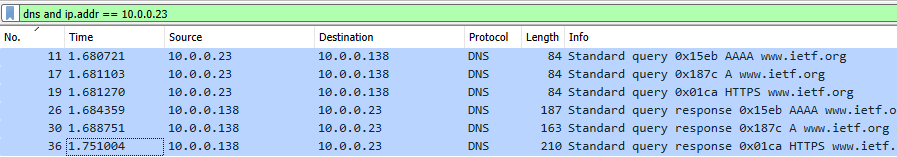
\includegraphics[width=1.2 \textwidth]{resources/dns1.png}\centering
	\end{center}
    On the server side the port was 53 in all of the packets (so 53 as destination of requests
    and as source of answers), and on the client side 3 different ports were used: 50883, 50884, 50885.
    \item The DNS queries had a source IP's of my ethernet adapter \texttt{10.0.0.23} and destination IP
    of the default gateway \texttt{10.0.0.138}, the answers to the queries had the source IP of the
    gateway and destination address of my ethernet adapter:
    \begin{verbatim}
    C:\Windows\System32>ipconfig
    ...
    Ethernet adapter Ethernet:

    Connection-specific DNS Suffix  . : home
    IPv6 Address. . . . . . . . . . . : 2a06:c701:7241:5300:95d8:e6b8:e777:abcf
    Temporary IPv6 Address. . . . . . : 2a06:c701:7241:5300:83d:935a:b003:26a5
    Link-local IPv6 Address . . . . . : fe80::940f:4df:377e:f2cb%21
    IPv4 Address. . . . . . . . . . . : 10.0.0.23
    Subnet Mask . . . . . . . . . . . : 255.255.255.0
    Default Gateway . . . . . . . . . : fe80::1%21
                                        10.0.0.138
    \end{verbatim}
    So this means that the default gateway is the DNS provider for my host system.
    \item Each of the 3 queries that were made had recived as single response to the port from
    which it was sent. Each such response contains a list of queries and responses.
    \item The query content for the query coming out of 50885:
    \begin{center}
        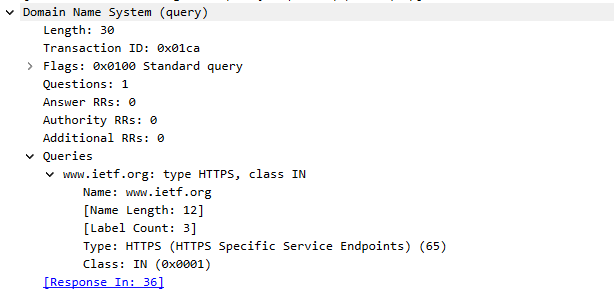
\includegraphics[width=1.2 \textwidth]{resources/dns3.png}\centering
    \end{center}
    And the response:
    \begin{center}
        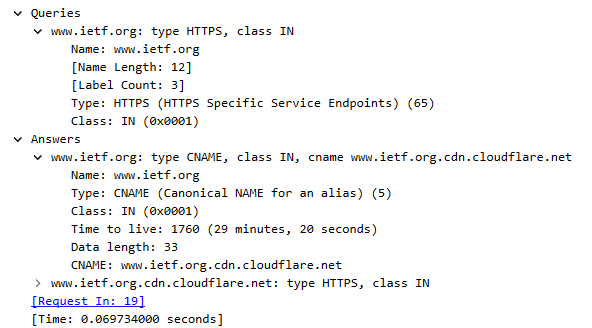
\includegraphics[width=1.2 \textwidth]{resources/dns2.png}\centering
    \end{center}
    \item The client port is 61983 while the server port is still 53.
    \item Like before, the DNS communication is between my computer and the default
    gateway. It is not a DNS itself - but acts as the DNS for my system.
    \item The request was of type 'A' which requests a host address.
    \item The response contained two host addresses,
    and a list of authoritative name servers.
    \item In this photo we can see to two relevant request and 
    response packets at the top, and also the content of the response packet below:
    \begin{center}
        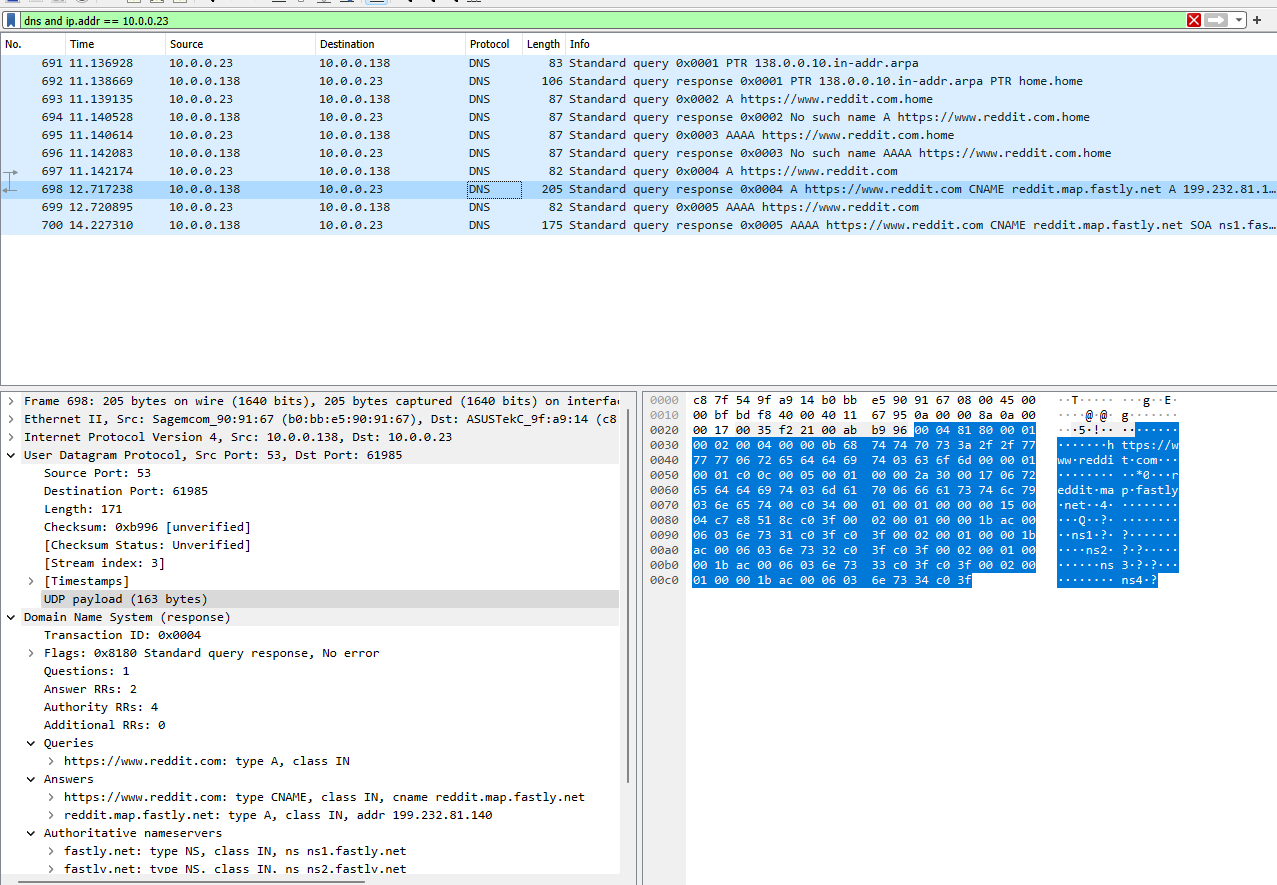
\includegraphics[width=1.2 \textwidth]{resources/dns4.png}\centering
    \end{center}
    \item The server address is still the default gateway.
    \item The query type is now 'NS' which means it is in search of a name server.
    \item There are 4 answers, all of them contain the of a name server, but none conain the IP itself.
    \item Wireshark:
    \begin{center}
        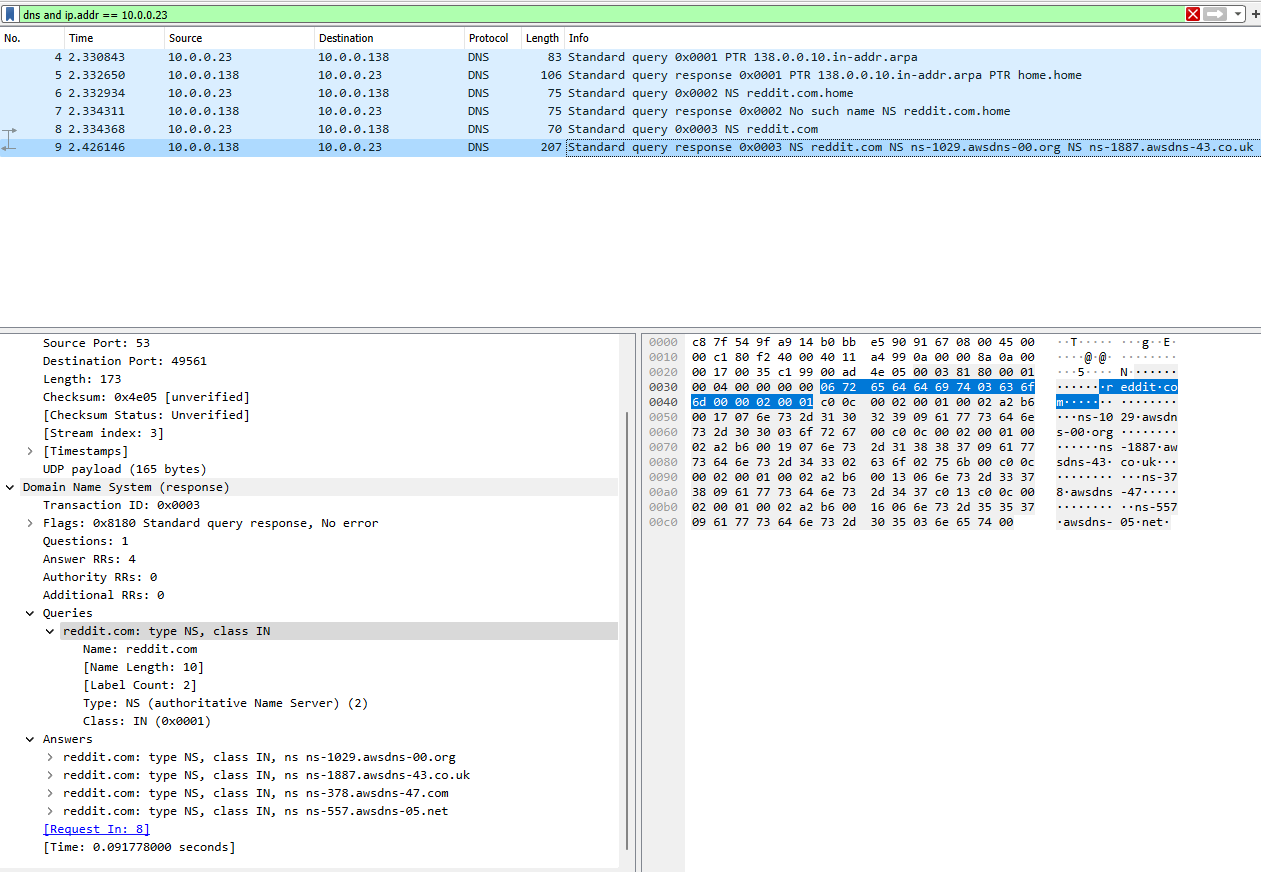
\includegraphics[width=1.2 \textwidth]{resources/dns5.png}\centering
    \end{center}
    \item A request to find who is \texttt{google-public-dns-a.google.com}.
    \item The request to find \texttt{google-public-dns-a.google.com} was sent to the default gateway. It is my local DNS provider.
    The response also came from the default gateway.
    \item The request to find \texttt{reddit.com} was sent to the address \texttt{2001:4860:4860::8888}
    which resolved address of \texttt{google-public-dns-a.google.com} (which is not my local DNS server).
    \item The IPv6 address of the google DNS server:
    \begin{verbatim}
    PS C:\Users\yosef> nslookup google-public-dns-a.google.com           
    Server:  home.home
    Address:  10.0.0.138

    Non-authoritative answer:
    Name:    google-public-dns-a.google.com
    Addresses:  2001:4860:4860::8888
            8.8.8.8
    \end{verbatim}
    Wireshark:
    response packets at the top, and also the content of the response packet below:
    \begin{center}
        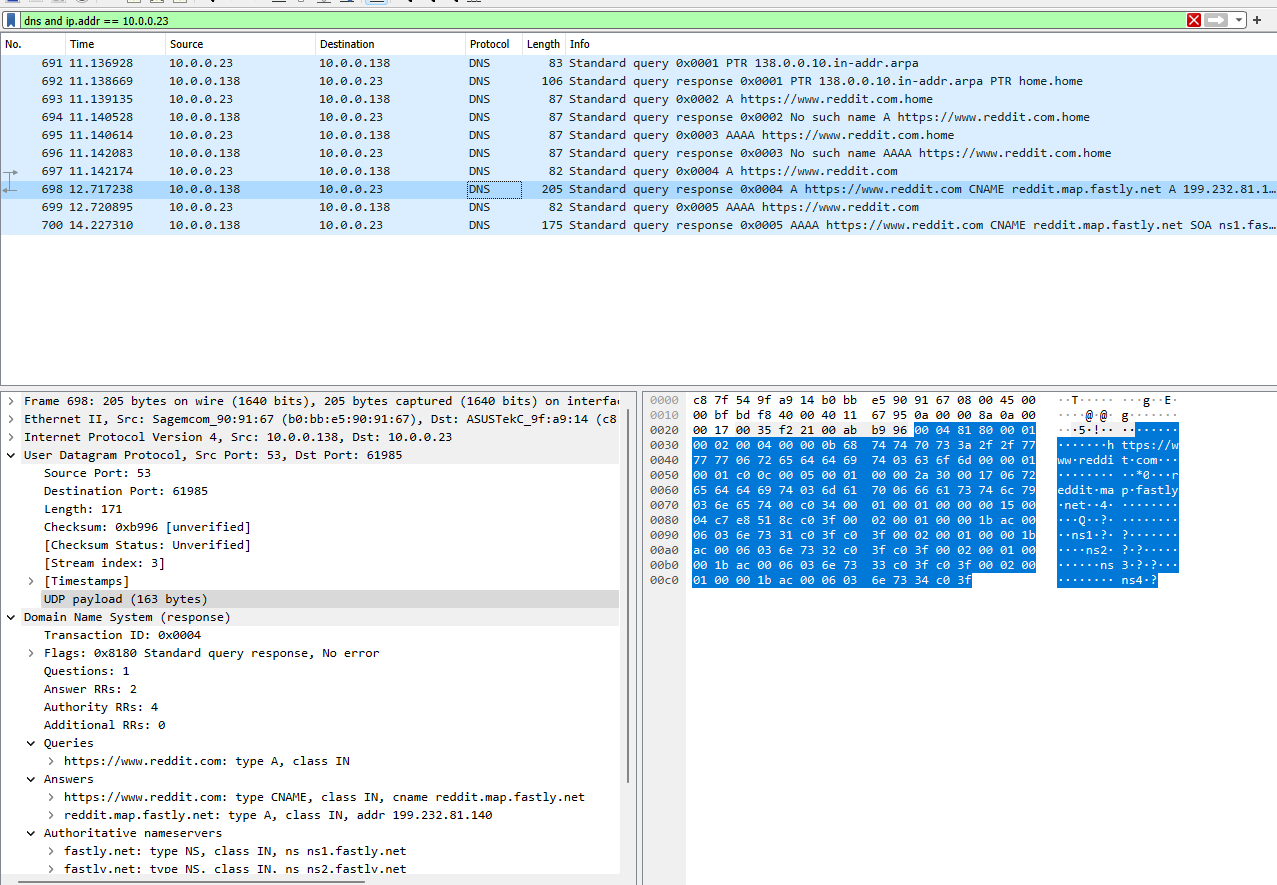
\includegraphics[width=1.2 \textwidth]{resources/dns4.png}\centering
    \end{center}


    
\end{enumerate}
